\subsection{Control of the car}
At the interview the costumers expressed that they needed to change how the car was controlled.
They wanted the car to reflect the current sound level of the speech recorded by the microphone.
This is expressed in requirement \ref{carcontrolReq} which is as follows:
\begin{enumerate}
\setcounter{enumi}{5}
\item The car is controlled in such a way, that the vertical position of the car is relative to the current loudness of the player's voice.
\end{enumerate}

This has been implemented in the game by mapping the values recorded by the microphone to a range that corresponds to the height of the screen.

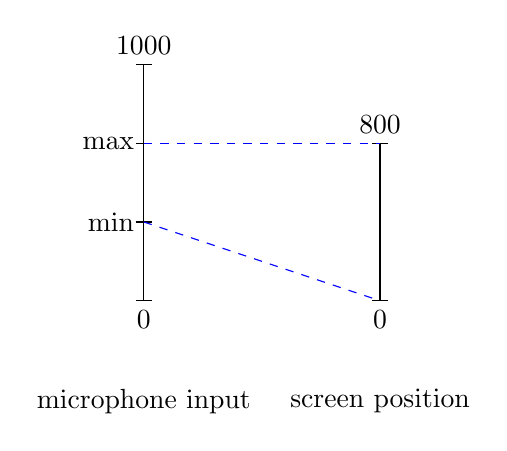
\begin{tikzpicture}
%vertical scales
\draw (0,0) -- (0,3); 
\draw (3,0) -- (3,2);

\node [below] at (0,-1){microphone input};
\node [below] at (3,-1){screen position};

%  endpoints with labels
\draw (-0.1,0) -- (0.1,0); 
\node [below] at (0,0){0};

\draw (-0.1,3) -- (0.1,3);
\node [above] at (0,3){1000};

\draw (2.9,0) -- (3.1,0); 
\node [below] at (3,0){0};

\draw (2.9,2) -- (3.1,2);
\node [above] at (3,2){800};

%min and max labels 
\draw (-0.1,1) -- (0.1,1);
\node [left] at (0,1){min};

\draw (-0.1,2) -- (0.1,2);
\node [left] at (0,2){max};

% mapping lines
\draw [dashed, blue](0,2) -- (3,2);
\draw [dashed, blue](0,1) -- (3,0);
\end{tikzpicture}